\chapter{Signal Analysis}
\label{Ch:SignalAnalysis} \lhead{Chapter 6. \emph{Signal Analysis}} % Write in
your own chapter title to set the page header

% what do I have
\section{Resonance} NOTE: maybe I should discuss RESONANCE in the physical
problem part...?

Resonance is an important phenomena in a number of engineering applications,
characterised by quantities such as resonant frequencies, quality factors and
mode shapes. The advantage of time domain simulations is that a broadband
frequency response can be obtained in a single run. However the the frequency
content isn't readily available and needs to be extracted from the obtained time
domain evolution of the system. In this chapter we will discuss the fourier
decomposition of the time domain solution using parametric and non-parametric
methods and the errors associated with this transformation.

\section{Introduction} ** what I have: a discrete-time signal - discrete in x,
continuous in y ** finite length ** discretely sampled ** time domain (function
of time) ** how this connects with resonance * Q: how can we turn the signal
which depends on time -> function that depends on frequency (spectrum) ** what
is a signal...?

\section{DFT} Introduce the inner product + ideas around projection.... % FROM
BEFORE>...! Fourier transform is a techniques which permits decomposition of any
time-domain signal into its frequency domain representation. Based on the
Fourier series in which a periodic time domain signal $s(t)$, with a period $T$
such that $s(x)=s(x+nT)$ for $n=1,2,3 ...$ can be written on the interval
$(-l,l)$ as

The Fourier transform of $s(t)$, denoted as $\hat{s}(f)$, is a complex function
of frequency whos magnitude and complex argument represent respectively the
amplitude and phase offset of the infinite series of sinosoidal functions of
which $s(t)$ is composed.

\section{Sinusoids} Complex/Real sinusoids...correspondance Equivalence of
sinusoids with same frequency (different phase)... justify that signals can be
expressed as a series of sinusoids
\subsection{Sinosuoidal Basis} Taking the discrete fourier transform corresponds
to the projection of the signal onto a basis of sinusoids of different
frequencies. It is well known that any two sinusoids, $\signonorthocont_1(t)$
and $\signonorthocont_2(t)$, of arbitrary phase and ampltude, defined on the
interval $t \in [-\infty, \infty]$, with frequencies $\omega_1$ and $\omega_2$
are orthogonal for any $\omega_1 \neq \omega_2$. For two discrete sinusoids,
$\signonortho_1(t)$ and $\signonortho_2(t)$ however, this condition only holds
for the frequencies which are periodic in $N$ samples. Consider a set of
discrete sinusoid $\{ \sig_f\}$, of frequency $\omega_f$, given by
$$
\signonortho_f(n) \equiv \frac{1}{\sqrt{N}}e^{i\omega_f n T}.
$$
where the factor $\sqrt{N}$ has been included for normalisation. The inner
product between two sinusoids from this set, $\sig_l$ and $\sig_m$, is given by
\begin{align} \left< \signonortho_f, \signonortho_k \right> &\equiv \invsqrN
\sum_{n=0}^{N-1} \signonortho_f(n) \overline{\signonortho_k(n)} \\ &= \invsqrN
\sum_{n=0}^{N-1} e^{i ( \omega_f - \omega_k) nT} \\ &=
    \begin{cases} \frac{N}{\sqrt{N}} & \textrm{for}\ \omega_f = \omega_k \\
\frac{ 1 - e^{i ( \omega_f - \omega_k) NT} }{ \sqrt{N} ( 1 - e^{i ( \omega_f -
\omega_k) T} ) } & \textrm{otherwise}
    \end{cases}
\label{eq:inner-product-general}
\end{align} where the final step is acheived by observing that a geometric
sequence $x(z_1) \equiv \sum_{n=0}^{N - 1} z_1^n$, can be written as $x(z_1)
\equiv \frac{1-z_1^N}{1-z_1}$ for any $z_1 \in \{\ \ComplexSet\ |\ z_1 \ne 1
\}$. Consider a subset, $\{ \sig_k \}$ of $\{ \sig_f \}$, with sinusoids of
frequency $\omega_k \equiv k \frac{2 \pi }{N} f_s$, for $k \in
\IntegerSet[0,N-1]$. It can be easily verified
from~\eqref{eq:inner-product-general} that the inner product between two members
of this set, $\sig_k$ and $\sig_l$, is given by
$$
\left< \sig_k, \sig_l \right> =
\begin{cases} \frac{N}{\sqrt{N}}, & \text{for}\ k = l \\ 0, & \text{for}\ k \ne
l
    \end{cases},
  $$
and are thus orthogonal to each other. It can also be readily verified from that
the norm of $\signonortho_k$ is given by
\begin{align*} \norm{\signonortho_k} &= \left< \signonortho_k, \signonortho_k
\right>^{1/2} \\ &= \left( \sum_{n=0}^{N-1} e^{j 2 \pi(k-k) n / N} \right)^{1/2}
\\ &= \sqrt{N}
\end{align*} It can be shown that $\{ \sig_k \}$ form an orthonormal, complete
basis\cite{} spanning $\ComplexSet^{N}$, in which any discrete, $N$-sampled
complex sinusoid can be expressed. We will describe $\{ \sig_k \}$ as the
\textit{ discrete Fourier basis }. Another thing....show that any x(t) is
expressable as a superposition of sinusoids....!? % equivalence for sinusoids
with different amplitude and, phase etc etc... % condition otherwise they're
equal % todo - this is for a specific cases...right? % unit amplitude, zero
phase complex sinusoids -> it is readily verified that % any nonzero amplitude
and phase have no effect on orthogonality. The projection of a discrete signal,
$\{ x(n) \} \in \ComplexSet^{N} $, onto the $k$th discrete Fourier basis
function, $\sig_k$, is given by % TODO: in the book it ISNT the orthonormal
basis thats used.... just the ortho one
\begin{equation} \Projection_{\sig_k} (x) = \frac{ \left< x, s_k \right>
}{\norm{s_k}^2} \sig_k \label{eq:projection-onto-basis}
\end{equation} The discrete frequency spectrum, $\Spectrum(\omega_k)$, is then
defined as the coefficients of this projection
\begin{equation} \Spectrum(\omega_k) \equiv \frac{1}{\sqrt{N}}\sum_{n=0}^{N-1}
x(n) e^{-i 2 \pi k n / N}\ \ \textrm{for}\ k = [0,N-1]
  \label{eq:dft} .
\end{equation} The correponding inverse transform, given simply by the sum of
the projections,
\begin{equation} x(t) = \frac{1}{\sqrt{N}} \sum_{k=0}^{N-1} \Spectrum(\omega_k)
e^{i 2 \pi k n / N}
  \label{eq:idft} ,
\end{equation} allows the original signal to be reconstructed from the spectrum,
$\{ \Spectrum(\omega_k) \}$. % have I dropped T here...?
Equations~\eqref{eq:dft} and~\eqref{eq:idft} are known respectively as the
discrete Fourier transform (DFT) and the inverse discrete Fourier transform
(IDFT) of $\{ x(n) \}$. The process of sampling a continuous signal and
transforming to a discrete frequency domain domain representation,
using~\eqref{eq:dft}, is referred to as Fourier analysis. The inverse process,
whereby an (approximation of) the original continuous signal is obtained from
the spectral components, $\Spectrum(\omega_k)$, using~\eqref{eq:idft} is
referred to as Fourier synthesis. % omega_k is discrete

% TODO - anything about periodic extension? assumption of periodicity? maybe put
% this in the spectral leakage section. % TODO - mention something about
amplitude and phase early -- and maybe state that in this case phase is not of
interest...? Put this gently. Careful with the word % BASIS written with the
same amplitude and phase (phase is necessary for orthogonality, amplitude for
normalisation).


\section{Shannon Theorem} \NiquistFreq define \omega_N as the niquist frequency.

\section{Spectral Leakage} % TODO: talk about periodic extension here.... A
continuous signal, $x(t)$, with a maximum frequency $\NiquistFreq$, and
periodicity which is an integer divisor of the sampling duration $T$, can
readily be expressed exactly as a linear superposition of continuous sinusoids
with the frequencies as the fourier basis, $\omega_k = 2 \pi k f_s / N$ for $k
\in [0,N-1]$. Therefore the original continuous signal $x(t)$ is reconstructed
exactly by Fourier synthesis of the Spectrum obtained by Fourier analysis. For a
signal which contains frequencies different from the basis frequency, this is
not the case. Whilst the continuous function obtained reproduces $x(t)$ exactly
at the $N$ sample points, it may differ away from these values. % IS THIS
TRUE....!??? I think so...!? Should verify this. Consider the projection of
$\{x(t)\}$ onto the discrete Fourier basis function $\sig_k$, where the
projection coefficients, from~\eqref{eq:inner-product-general}, are given by
\begin{align*} \Spectrum(\omega_k) &=\equiv \frac{ 1 - e^{i (\omega_f -
\omega_k) N T} }{1 - e^{i(\omega_f - \omega_k) T}} \\ &= \frac{ \sin[(\omega_f -
\omega_k)N T / 2]}{\sin[(\omega_f - \omega_k) T / 2]} e^{i (\omega_f - \omega_k)
(N - 1) T /2}
\end{align*} which is equivalent to the contribution of an arbitrary frequency
$\omega_f$ to the $k$the spectrum of the signal. A plot of the amplitude of the
contribution against the frequency of the sinusoid is given
in~\ref{fig:amplitude-contribution-to-component-by-freq}.
\begin{figure}[h] \centering
  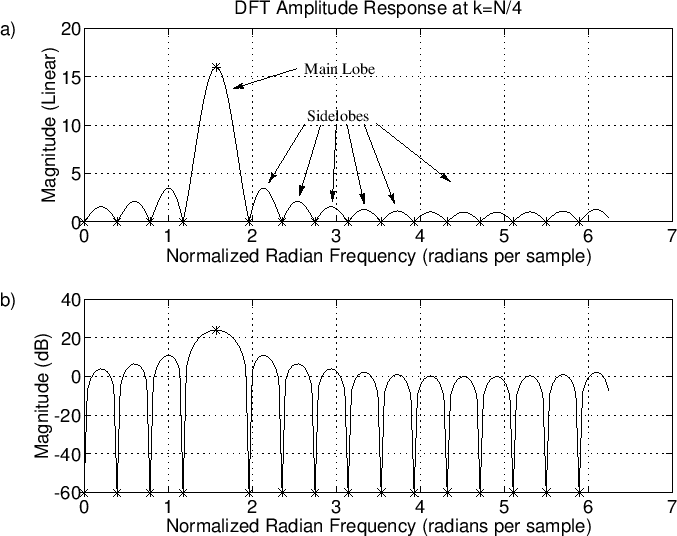
\includegraphics[width=\textwidth]{Figures/Chapters/SignalAnalysis/img1065}
  \caption{Plot showing the amplitude contribution of a sinusoid at any
frequency \omega_f to a given spectral component}
  \label{fig:amplitude-contribution-to-component-by-freq}
\end{figure} The largest contribution to $\Spectrum(\omega_k)$ comes from the
frequency of the basis, $\omega_k$, and contributions from the other basis
frequencies $\omega_l$ where $l \in { \IntegerSet\ |\ l \ne k}$ is zero, as is
expected since functions are orthogonal. However it can be seen that frequencies
between basis function frequencies have a non-zero contribution to the
$\Spectrum(\omega_k)$, with the frequencies in the frequency bin between
$\omega_{k-1/2}$ to $\omega_{k+1/2}$ contributing the most. However we see that
$\Spectrum(\omega_k)$ is sensitive to all frequencies between $\omega_0$ and
$\omega_N$. This phenomena is known as \textit{spectral leackage} and is due to
discontinuites caused by periodic extension of functions which do not exhibit a
periodicity $T$, and is exhibited by all frequency components except for $\{
\omega_k \}$. Note that peak spectral leakage is caused by truncation of the
signal at the endpoints of the sample window, and is not reduced by increasing
$N$\cite{}. % TODO - more on input signal being the same as its extension ->
Section 7.1.2

The contribution which a frequency makes to further frequency components can be
minimised by an appropriate choice of window function. Such window functions
will go to zero at the endpoints of the interval, thereby producing a signal
with periodicity $T$. This has the effect of widening the main lobe and reducing
the amplitude of the side lobes compared to the leakage of a rectangualar wave
shown in~\ref{fig:amplitude-contribution-to-component-by-freq}. % MODFT: more
about this in Chapter 8 (apparently) % why doesn't this remove leakage
completely. %%% The window function will %%% -> addition of sinc wiggles... %%%
Since multiplication by of corresponds to multiplication in the Fourier domain
%% need to include more terms... In realistic broad band applications, a
sufficiently large $N$ to be periodic for all frequen in fact not periodic in
$N$ or aperiodic. and periodic extension of these signals would result in a
discontinuity. , or equivalently are finite signals of length $N$, periodically
extended with period $N$. ** for signal of finite length ** for signal sampled
at discrete times ** classification -> continous time, discrete time,
digital(but not necessary) % MORE STUFF... finite signal -> window (our signal
is a representation of a longer time domain signal) issues with rectangular
window(s) is this general? or a property of DFT? or a property of finite
signals...?

rectangular window -> sinc function -> spectral leakage words: truncation
artefacts or sinc wiggles

methods (supposedly) designed to reduce truncation * maxiumum entropy * linear
prediction * FDM % thats what it says in
http://www-keeler.ch.cam.ac.uk/lectures/understanding/chapter_4.pdf


* example of what a spectrum looks like * what are the peaks, what is resonance
etc * Quantities of interest * Peak height * Peak width (Quality factor
calculations) * FSR * phase

% FOLLOWING IS FROM PREVIOUS WRITING...IS IT TRUE FOR DFT? The continuous
fourier transform requires that integration is preformed between $-\infty$ and
$\infty$, or over an integer multiple of the periodicity of the signal, $T$. For
most sampled signal with multiple frequency components it is not possible in
general to measure signals which would be repeated periodically in $T$. That is
signals where $s(T) = s(0)$. Such signals extended to infinity would exhibit
discontinuities. These discontinuities give rise to a phenomena known as
spectral leakage[], in order to capture these discontinuities, which introduces
noise into the system. This is clearly not desirable, and can be reduced by
using a window function, such as the Blackman window. The signal is multiplied
by and envelope which ensures the discontinuity is eliminated. * Show some
examples of spectral leakage and how it can be handled...
\section{Linearity} It can be shown easily verified that taking the discrete
Fourier transfrom is a linear operation. For any $x,y \in \ComplexSet^{N}$ and
any $\alpha,\beta \in \ComplexSet$ the DFT transform satisfied
$$
\alpha x + \beta y \to \alpha X + \beta Y
$$
since,
\begin{align*} DFT_k &\equiv \sum_{n=0}^{N-1} \left[ \alpha x(n) + \beta y(n)
\right] e^{-j 2 \pi n k / N} \\ &= \alpha \sum_{n=0}^{N-1} \alpha x(n) e ^ {-i 2
\pi n k /N} + \beta \sum_{n=0}^{N-1} y(n) e^{-i 2 \pi n k / N} \\ &\equiv \alpha
X + \beta Y
\end{align*} where $X$ and $Y$ are respectively the discrete fourier transforms
of $x$ and $y$. ** also the maxwells equations are linear....so extra linearity

\section{Spectrum Symmetry} In our case, we are interested on in only real input
signals where $x \in \Real^N$. In this case the spectrum can be written as
\begin{align*} \Spectrum(-k) &\equiv - \DFTsum x(n) \DFTexp{( -k )} \\ &=
\overline{ \DFTsum \overline{x(n)} \DFTexp{k}} \\ &= \overline{ \DFTsum x(m)
\DFTexp{k}} \\ &= \overline{\Spectrum(k)}
\end{align*} For a real signal, $\RealPart{\Spectrum(k)}$ and $|\Spectrum(k)|$
are even symmetric functions and $\ImagPart{\Spectrum(k)}$ and $\angle
\Spectrum(k)$ is an odd symmetric function. Due to this symmetry, only positive
frequencies (from $0$ and $\fs/2$) are plotted when presenting spectra, since
negative frequencies contain no additional information. % TODO - be more
specific about what is meant by FLIP(x) or x(-n)... % note, I haven't proved
that the angle or magnitude are even/odd here...but it follows from conjugate
summetry of X in polar form X(k) = |X(k)|e^{i \angleX(K)} i.e. just write X(k)
in polar form and its immediately obvious...is it?
\begin{align*} DFT_k(-x) &\equiv \DFTsum x(N-n) \DFTexp{k} \\ &=
\sum_{m=0}^{N-1} x(m) e^{- i 2 \pi (N-m)k / N} \\ &= \sum_{m=0}^{N-1} x(m) e^{-
i 2 \pi m ( -k ) / N} \\ &\equiv \Spectrum(-k)
\end{align*} Therefore for any real signal reversal of the signal in time leads
to reversal of the spectrum.
\begin{quote} Definition: A signal with a real spectrum (such as any real, even
signal) is often called a zero phase signal. However, note that when the
spectrum goes negative (which it can), the phase is really $ \pm\pi$ , not 0 .
When a real spectrum is positive at dc (i.e., $ X(0)>0$ ), it is then truly
zero-phase over at least some band containing dc (up to the first zero-crossing
in frequency). When the phase switches between 0 and $ \pi $ at the
zero-crossings of the (real) spectrum, the spectrum oscillates between being
zero phase and ``constant phase''. We can say that all real spectra are
piecewise constant-phase spectra, where the two constant values are 0 and $ \pi
$ (or $ -\pi$ , which is the same phase as $ +\pi$ ). In practice, such
zero-crossings typically occur at low magnitude, such as in the ``side-lobes''
of the DTFT of a ``zero-centered symmetric window'' used for spectrum analysis
(see Chapter 8 and Book IV [73]).
\end{quote}

\begin{itemize}
\item shift theorem -> a delay in time domain corresponds to a linear phase term
in the frequency domain -> spectral magnitude unaffected by a linear phase term
\item zero phase signals
\end{itemize}

\section{Parsevals Theorem}
\begin{itemize}
\item interpretation as energy per bin...
\end{itemize}

\section{Zero Padding \& Interpolation}
In most cases its not practical to collect a signal for sufficiently long
time to reach the required error in frequency. A method of interpolation is desired. As we will see appending zeros to a causal signal (that is a signal which is zero before t=0), corresponds to ideal interpolation in the frequency domain. Let $y \in
\ComplexSet^{M}$ be a signal of length $M$, obtained by padding a signal $x \in
\ComplexSet^{N}$ with zeros, such that
\begin{align*} y(m) =
  \begin{cases} x(m) & \textrm{for}\ m \in [0,N-1] \\ 0 & \textrm{otherwise}
  \end{cases}
\end{align*} The DFT of $y$ is then given by
\begin{align*} DFT_k(y) &= \sum_{m=0}^{M-1} y(m) e^{- i 2 \pi m k' / N} \\ &=
\sum_{n=0}^{N-1} x(n) e^{- i 2 \pi n k' / N} \\ &= \Spectrum(\omega_{k'})
\end{align*} where $\Spectrum(\omega_{k'})$ is in fact the projection
coefficient of the signal $x(n)$ onto a discrete Fourier transform sinusoid of
frequency $\omega_{k'}$. This is exact for a time-limited signal, which is truly
zero outside of the window.
% VIVA / TODO :what about non-time-limited????
Note that interpolation will not improve resolution in the sense of being able to resolve closely spaced peaks.

Since the FFT algorithm allows the DFT of spectra to be computed quickly and
effective, padding the time domain signals with zeros prior to and FFT is an
efficient way of interpolating a spectrum. However, for a given accuracy, this
method is often more computationally expensive than padding the signal with a
smaller number of zeros, and performing a quadratic interpolation of the
spectrum amplitude in the vicinity of a peak. We refer to this as the
quadratically interpolated FFT (QIFFT) method~\cite{}
% https://www.dsprelated.com/freebooks/sasp/Sinusoidal_Peak_Interpolation.html
In quadratic interpolation of sinusoidal spectrum-analysis peaks, we replace the main lobe of our window transform by a quadratic polynomial, or ``parabola''. This is valid for any practical window transform in a sufficiently small neighborhood about the peak, because the higher order terms in a Taylor series expansion about the peak converge to zero as the peak is approached.

Note that, as mentioned in §D.1, the Gaussian window transform magnitude is precisely a parabola on a dB scale. As a result, quadratic spectral peak interpolation is exact under the Gaussian window. Of course, we must somehow remove the infinitely long tails of the Gaussian window in practice, but this does not cause much deviation from a parabola, as shown in Fig.3.36.

values in the vicinity of the peaks. Since this is 

given accuracy, o

Since FFTs are efficient, this is an efficient interpolation method.
However, in audio spectral modeling, there is usually a limit on the needed
accuracy due to the limitations of audio perception.
As a result, a ``perceptually ideal'' spectral interpolation method that is even more efficient is to zero-pad by some small factor (usually less than 5), followed by quadratic interpolation of the spectral magnitude. We call this the quadratically interpolated FFT (QIFFT) method [271,1]. The QIFFT method is usually more efficient than the equivalent degree of ideal interpolation, for a given level of perceptual error tolerance (specific guidelines are given in §5.6.2 below). The QIFFT method can be considered an approximate maximum likelihood method for spectral peak estimation, as we will see.
% VIVA: what does this mean

For a time-limited signal, which is zero outside of the measurement window, this
is


For time-limited this is idea, since the signal is zero outside of the
window....for non-time limited signals (like mine)...what happens...? Such
spectral interpolation is ideal when the closely spaced spectrum points. spacing
of . We define the zero padding operator


a causal signal with frequencies are within the desired resolution of the actual
frequencies. ** note: padding with zeros apparently is the same as spectral
interpolation -> this SHOULD actually be pretty good...no? - the only
disadvantge, is I'm now taking the DFT of something which is not the original
signal... ** note: zero padding should be done BEFORE windowing... ** note:
apparently this is independent of the weird window effects I get...? ** there is
also such a thing as ``upsampling'' - alternative approach

Stack Exch Zero-padding in the time domain corresponds to interpolation in the
Fourier domain. It is frequently used in audio, for example for picking peaks in
sinusoidal analysis. While it doesn't increase the resolution, which really has
to do with the window shape and length. As mentioned by @svenkatr, taking the
transform of a signal that's not periodic in the DFT size is like multiplying
with a rectangular window, equivalent in turn to convolving it's spectrum with
the transform of the rectangle function (a sinc), which has high energy in
sidelobes (off-center frequencies), making the true sinusoidal peaks harder to
find. This is known as spectral leakage. But I disagree with @svenkatr that
zero-padding is causing the rectangular windowing, they are separate issues. If
you multiply your non-periodic signal by a suitable window (like the Hann or
Hamming) that has appropriate length to have the frequency resolution that you
need and then zero-pad for interpolation in frequency, things should work out
just fine. By the way, zero-padding is not the only interpolation method that
can be used. For example, in estimating parameters of sinusoidal peaks
(amplitude, phase, frequency) in the DFT, local quadratic interpolation (take 3
points around a peak and fit a parabola) can be used because it is more
computationally efficient than padding to the exact frequency resolution that
you want (would mean a much larger DFT size).

--> zero padding is basically interpolation in frequency domain...! -->
alternative is local quadratic interpolation

ZERO PADDING -> INTERPOLATION (from book)

QIFFT (quadratic interpolation FFT)
review paper (I think) https://ai2-s2-pdfs.s3.amazonaws.com/7bbc/c4d13458d0a6570fba35f508c2b44444fb07.pdf
also a paper to reference (for quadratic interpolation FFT)
 M. Abe and J. O. Smith, “Design criteria for simple sinusoidal parameter
estimation based on quadratic interpolation of FFT magnitude
peaks,” in 117th Audio Engineering Soc., 2004, Paper no. 6256.



\section{Better than FFT...}
http://researchrepository.napier.ac.uk/4022/1/phd.pdf [p.43] <- some references
here parametric approaches - what are these? non-parametric approaches - what
are these?

\section{FWHM -> decay time} Conversion between FWHM and decay time
http://physik.uni-graz.at/~atr/publications/phd-thesis.pdf [p.189]

\section{Sampling Theorem}

Claude Shannon -> sampling theorem (best known)

continuous time signal $x(t)$ with highest freq $\fmax$

sample it periodically at a rate $f_s = 1/T_s > 2*f_max$, then the signal is
exactly recovered from $\{x[k]\}$ the sampled values, using the interpolation
rule:
$$
x(t) = \sum_{k=-\infty}^{\infty} x(k \Ts) h(t - k \Ts)
$$
where
$$
h(t) = \frac{sin(\pi t / \Ts)}{\pi t / \Ts}
$$

** Aliasing (alias...! non-unique...!)


\section{Spectrum} FROM BEFORE: A correctly scaled fourier transform of a time
domain signal is known as the power spectrum of the signal. real part ->
absorption mode line - in fact, in the case of exponential decaying signal, such
as
$$
  S(t) = S_0 e^{i \omega t}exp^{ -R_2 t }
$$
$R_2 = 1 / T_2$ rate constant, larger rate constant -> more rapid decay $T_2 = $
time constant, the shape of the line is known as a Lorentzian, 'or to be precise
the absorption mode Lorentzian' ....> What is this absorbtion mode stuff? %
http://www-keeler.ch.cam.ac.uk/lectures/understanding/chapter_4.pdf

'The imaginary part of the spectrum gives a lineshape known as the dispersion
mode Lorentzian'

Absorbtion Lorenzian shape (show it) -> Integral/area is constant width = half
the max height --> broader and shorter, narrower and taller something to do with
height being $1/(\pi T_2)$ Hz % why Hz ??? Height directly proportional to
amplitude...

Dispersion Line obviously the integral thing isn't true any more... also broader
than the absorption mode... %note Dispersion line ISNT realted to derivative
line of ESR spectra

Fourier transform is linear process, so
\begin{equation} \FT{a x(t) + b y(t) } = a \FT{x(t)} + b \FT{y(t)}
\end{equation} for any time domain functions $x(t)$ and $y(t)$.

Also, time shift:
$$
\FT{x(t \pm t_0)} = \FT{x(t)} e^{\pm i \omega t_0}
$$

if sig is a sum of decaying terms, then total FT will be the sum of the line
corresponding to each peak -> this is actually useful with max frequency

** Phase -> what is the phase? what does it correspond to? how does it
correspond to the imaginary part of FFT? Is it useful? (dont think so???)
Interesting -> by shifting the phase of the wave I can swap the real and
imaginary parts of the FT...? Is that true in my case..?

after signal has decayed -> just recording noise --> reducing the time, mean
better signal to noise ratio (SNR) --> but also means that not as much signal
produced --> careful with this ----> Excitation is used instead time spend
recording signal == aquisition time (is this a real term?)

Sensitivity enhancement: Signal is strongest initially, and decays --> first
part is ``more important'' --> multiply by a decaying function (1 -> 0) -->
weighting gives more importance to early stuff ---> not (I think) this also
affects amplitude...so should point this out.

Example weighting function:
$$
W(t) = exp(-R_{LB} t)
$$
where $R_{LB} = $ rate constant (choice).

Different $R_{LB}$ changes noise + also changes amplitude (so I need to
normalise back, also amplitude meaning is lost -> which is kinda true anyway,
right?)

Note: weighting function will also broaden the lines (since decay is happening
quicker) and reduce peak height...!

NOTE: by taking the absolute value, actually I don't care about phase any more,
because the absolute value doesn't vary with phase % check that it IS the
absolute value that I should be taking Complex -> phase + magnitude Signals
'power' in a frequency bin = amplitude (ish - not sure about this)

Question: is my Lorentzian the shape of the amplitude or the shape of the real
part that is in phase? Are these two thing equivalent? Does fitting with a
Lorentzian imply that I need to use the real part of the spectrum?

Question: maybe a better way to think about this is the absolute value and phase
angle...?

\section{FFT} * present FFT as a way of computing DFT * who came up with it *
how important is it * how much faster is it * we don't have anything faster for
a GENERAL signal

\section{Alternatives} * These work for SPECIFIC cases.... STFT (short time fast
fourier transform) -> at least get a reference and some comments with reference
to existing work % --
http://repository.cmu.edu/cgi/viewcontent.cgi?article=1065&context=dissertations
z-transform - smaller windows spare FT - zero outputs (not intersting I don't
think) FDM - constrained to decaying outputs (solve eigenvalue problem)


\section{Obtaining Resonant Frequencies} * what is resonance and how do we
obtain it from the spectrum A system exhibits resonance if frequency components
at the resonant frequencies of the system oscillate with larger amplitudes than
away from these resonant frequencies. In this case peaks in power spectrum will
be seen at the corresponding resonant frequencies. Resonant frequency values can
be recovered by peak fitting. [ mention Lorentz fitting here? compare to spline
fitting? ]

* mention

*** Fast Fourier Transform ***

The widely used Fast Fourier transform [***] algorith which reduces the
computational of the DFT from an $\bigO(n^2)$ operation to an $\bigO(n log n)$
operation.

A discrete fourier transform of a time domain signal leads to a frequency domain
spectrum, where an amplitude is associated with evenly spaced, discrete points
in a frequency interval. This frequency domain representation of the signal is
exact provided that the number of point...***

This frequency amplitude is a complex number denoting the coefficient a given
frequency in the discrete fourier series expansion. This can be convieniently
plotted in an amplitude against frequency plot known as a power spectrum, where
the peaks of the spectrum corrispond to the resonant frequencies of the system.

The frequency resolution of the spectrum, that is the spacing of the discrete
points in frequency space, is given by

$$
\Delta f = \frac{1}{T}
$$

where $T$ is the final time of the simulation. Care should be taken to ensure
that the final time of the simulation is sufficiently long to account for the
desired simulation error.

% *** I can show this by showing in the results section how closely this matches
the actual error found


The maximum frequency, $f_{max}$, which can be resolved by a fourier transform
is given by the Niquist-Shannon theorem which states
$$
f_{max} \leq \frac{1}{2 \Delta t_s}
$$

where $\Delta t_s$ is the time between sampling points of the signal, the
sampling interval. A time domain signal in which the highest frequency component
has a frequency less that $f_{max}$ is represented fully by the frequency domain
spectrum. For time domain signals containing components of higher frequency that
$f_{max}$ *** aliasing ***. % what happens here...!? Clearly the simulation time
step, $\Delta t$, gives an upper limit on the sampling interval - therefore care
should be taken to choose the $\Delta t$ of the simulation to be sufficiently
small to allow the desired $f_{max}$ and also to allow for a sufficiently small
error in the time domain signal. Which of these criteria is limiting factor will
in general depend on the frequencies of interests.

\section{Resonant Frequencies}
\section{Mode Shapes}

The fourier transform can be thought of as a factorisation of the signal into a
temporal and spatial part. For a single point the spatial part will simply be a
complex amplitude. However when the entire domain is considered each point has
an associated complex amplitude for each frequency, which forms a spatial
envelope which when multipled by the temporal part defines the oscillations
associated with that frequency. When the frequency considered is a resonant
frequency, then the envelope is known as the mode shape associated with that
frequency.

\section{Quality Factors}

The quality factor is a widely used in engineering to describe the damping of an
oscillating system. The qaulity factor, $Q$, indicates the rate at which energy
is dissipated in the system. In applications where resonance is required,
engineering a system with a high-Q is usually desirable. In a high-Q system
resonant frequency oscillations will have a longer lifetime and less energy need
be provided to the system to maintain an oscillation. The Q-factor at a resonant
frequency, $f_{res}$ commonly written as the ratio

$$
Q = f_{res}/\B_{FWHM}
$$

where $B_{FWHM}$ is the bandwith of the resonant oscillation at half of its
amplitude, commonly known as the full-width-half-maximum (FWHM) value. An
equivalent definition can be given in terms of the ratio of energy stored in the
oscillator at resonant frequency to the rate of energy loss per cycle

In a resonant optical cavity the quality factor, $Q$, for a given resonant
frequency, $f_{res}$, is given by

$$
Q = 2 \pi f_{res} \frac{\Epsilon}{P}
$$

where $\Epsilon$ is the energy stored in the system and $P$, the dissipated
power, is given by $-\frac{d \Epsilon}{dt}$.

In resonant system with a high quality factor, resonant frequency oscillations
with have a long lifetime. Whilst oscillations away from the resonant frequency
will die out quickly. Conversely in a system with a lower Q-factor the resonant
oscillations will die out quickly and the resonant peak will have a larger
bandwidth. Figure \ref{fig:signal-analysis-low-vs-high-q-spectrum} shows the
resonant peaks of a circular PEC cavity, with a high quality factor, and the
same signal with dissipation introduced, that is a low quality factor.

\begin{figure}
\begin{center}
    \includegraphics[scale=]{Figures/SignalAnalysis/lowVsHighQualitySpectrum}
\end{center}
\caption{}
\label{fig:signal-analysis-low-vs-high-q-spectrum}
\end{figure}

For a dispersive system this will manifest itself in a wider spectrum line width
[], and consequentially a larger error in the quality factor. Note that
dispersion could be either physical or could be a non-physical dispersion
introduced by a numerical method.

A system with PEC boundaries and no material loss with no numerical errors is
expected to have a zero linewidth and infinite quality factor.

%WWWIIK

% *** maybe mention Q-switching - how does Q-switching work? Am I going to
research it?

\section{Envelopes} Since the signals being considered are of finite length, the
periodic repetition of a finite signal results in a discontinuity, unless the
final and initial values of the signal match exactly. This gives rise to a
phenomena called spectral leakage, where non-physical non-zero spectral
amplitudes are observed. For example consider a signal consisting of a single
frequency

$$
f(x) = sin(i2 \pi f_{res} x)
$$
.

Then taking a discrete Fourier transform of the signal over a finite interval
leads to spectral leakage as illustrated in figure
\ref{fig:signal-analysis-speactral-leakage-sine-wave}. Note that for longer
periods, less leakage occurs. Also note that figure {***} has significant lower
leakage than figure {***} with a similar signal length. This is due to the
signal in figure {***} having an integer multiple of cycles, resulting in a
signal which can be repeated periodically exactly.

\begin{figure}
\begin{center}
    \includegraphics[scale=]{Figures/SignalAnalysis/spectralLeakageSineWave}
\end{center}
\caption{Fourier transform of a number of sine waves with different intervals}
\label{fig:signal-analysis-speactral-leakage-sine-wave}
\end{figure}


These non-physical frequencies due to a finite interval can be reduced by
multiplying the signal by a suitable window function prior to performing the
DFT. This ensures that the initial and final values are zero. % This will
introduce an additional periodicity the length of the signal... There are a
number of choices of window, which should be selected according to the expected
frequency content of the time domain signal. We use the popular Blackman
envelope [***] prior to Fourier transforms in all examples in this work, unless
specified otherwise. The Blackman envelope is given by % REF: Blackman, R. B.
and Tukey, J. W. "Particular Pairs of Windows." In The Measurement of Power
Spectra, From the Point of View of Communications Engineering. New York: Dover,
pp. 98-99, 1959.
$$
A(x) = \frac{21}{50} \frac{1}{2} cos ( \frac{\pi x}{a} ) + \frac{2}{25} cos (
\frac{2 \pi x }{a} )
$$

A short sample signal with a filter applied is shown for illustration in figure
\ref{fig:signal-analysis-blackman-envelope}, alongside examples of spectra
obtained from the same signal with and without the filter to illustrate the
spectral leackage effect.

\begin{figure}
\begin{center}
    \includegraphics[scale=]{Figures/SignalAnalysis/blackmanEnvelope}
\end{center}
\caption{Blackman envelope applied to a superposition of two sin waves + the
spectrum of the superpositionof two sine waves of frequencies *** and *** with
and without a blackman filter applied }
\label{fig:signal-analysis-blackman-envelope}
\end{figure}

Figure \ref{fig:signal-analysis-comparison-of-envelopes} show the spectrum of
the same time domain signal alongside the spectrum shown after applying a number
of popularly used filters and the shape of these filters.

\begin{figure}
\begin{center}
    \includegraphics[scale=]{Figures/SignalAnalysis/comparisonOfEnvelopes}
\end{center}
\caption{}
\label{fig:signal-analysis-comparison-of-envelopes}
\end{figure}

\section{Need to explain the whole end to end process}

%% : possible comparison of different
\section{Zero frequency} If the frequency does not osciallate about zero, this
will manifest itself in the spectrum as a peak centered on zero. This will occur
of example when in a non-dissipative case the signal is sampled near a point
where the cavity was excited. It is therefore advisable when possible to pick a
point to sample a signal which is far from the source point.

\section{Fitting Parameters}

Lorenzian fitting assume a shape of the wave as

$$
e^{.../\tau}
$$

transformed into frequency space. We can use a Lorenzian fitting with a least
squares approach to obtain a good fit for a peak - provided that the peak is
isolated. However if the peak is near other peaks this can become a problem.

%some solution would be required to fit the lorenzian to the peak.

\section{Parametric Methods}

Parametric methods such as the filter diagonalisation method (FDM) use an
assumption of the shape of the signal to find the resonant frequencies by
solving an eigenvalue problem. This method can be used to significantly reduce
the error in the number time steps required to reach a solution. In numerical
experiements a increase of an order of mangnitude was observed for FDM over FFT.

However parametric methods are sensitive to dispersion which can degrade the
signal amplitude for signals which are of a considerable length, and therefore
while a better result can be obtained for a short run, for longer runs required
to obtain a high accuracy the method is unsuitable.

\begin{itemize}
  \item present the basis of the FFT method
  \item dependence of resolution/cut-off
	\item window functions / blackman envelope
	\item filter diagonalisation method
	\item Modal Shapes - how to obtain modes from resonant frequencies
  \item comparison of the FFT + FDM
  \item Summary of complete methods to recover resonant frequencies for a given
problem
\end{itemize}


%%% Local Variables:
%%% mode: latex
%%% TeX-master: "../Thesis"
%%% End:

